\documentclass[9pt]{IEEEtran}

\usepackage[english]{babel}
\usepackage{graphicx}
\usepackage{epstopdf}
\usepackage{fancyhdr}
\usepackage{amsmath}
\usepackage{amsthm}
\usepackage{amssymb}
\usepackage{url}
\usepackage{array}
\usepackage{textcomp}
\usepackage{listings}
\usepackage{hyperref}
\usepackage{xcolor}
\usepackage{colortbl}
\usepackage{float}
\usepackage{gensymb}
\usepackage{longtable}
\usepackage{supertabular}
\usepackage{multicol}
\usepackage{tabu}


\usepackage[utf8x]{inputenc}

\usepackage[T1]{fontenc}
\usepackage{lmodern}
\input{glyphtounicode}
\pdfgentounicode=1

\graphicspath{{./figures/}}
\DeclareGraphicsExtensions{.pdf,.png,.jpg,.eps}

% correct bad hyphenation here
\hyphenation{op-tical net-works semi-conduc-tor trig-gs}

% ============================================================================================

\title{\vspace{0ex}
Web crawler}

\author{Timotej Kovač\vspace{-4.0ex}}

% ============================================================================================

\begin{document}

\maketitle

\section{Introduction}

In this paper we present the structure, challenges and results of a web crawler implementation in Java.
It was used to crawl the *.gov.si websites and produced some interesting results.

\section{Web crawler}

\subsection{Implementation}

For the implementation of the web crawler we used Java and the following support libraries:
\begin{itemize}
\item{Jauntium (which uses Jaunt and Selenium libraries) in order to retrieve web pages and process them using a browser driver and so can also process JavaScript code~\cite{jauntium},}
\item{Robots which is used in order to process the robots.txt files for the domains that will be crawled~\cite{robots_txt}, }
\item{PostgreSQL which is used to connect and modify the postgres database~\cite{postgres}.}
\end{itemize}

Some other libraries have also been included mostly because the above mentioned ones depend on them.

The frontier is a list that consists of URLs that have yet to be visited.
The initial frontier consists of the starting URLs (see section Constants and issues).
It mainly behaves as a FIFO queue.
But because of the delay limitations that the crawler must obey the process of removing an URL starts as FIFO but skips every record that is not permitted to be visited at this time.

The crawling process begins with the initialization of multiple workers on separate threads which then start the process of crawling.
First they gain access to a locked frontier from where they take an available URL that has not yet been processed.
Then they update the next permitted window when the domain can be accessed again and proceed with the link processing.

First the program tries to send a HEAD request to get the content type of the target URL.
Because this part of the code offers a much more low level response then when using Jauntium the following redirects must be followed which happens in recursion.
Every URL is here also checked if it has been already crawled and if so the algorithm ends.
If not the data type is extracted from the head of HEAD request or the extension of the URL itself.

The next step is left to the Jauntium to visit the website and it to finish rendering the web page.
The permitted time for fetching is set to 5000 ms and the time to finish the loading of the web site is another 3000 ms. 

After that the text content of the website is processed so that all of the white space characters are removed. 
If this content matches any other web site in the database the algorithm ends.
If not the websites record in the database is updated with the retrieved information.

The next step are the links and images extraction.
Links are extracted from the website and are added to the frontier if multiple conditions are met.
Some of these are that the URL is a valid URL and not a JavaScript code or anything else, that we haven't visited it yet, that we can visit it based on the robots.txt permissions and so on.
Images are extracted as well and only their source address is added to the database.

After that all of the links that have been extracted are added to the database as well and the crawler thread starts the process again for the next link that is available in the frontier.

\subsection{Parameters and issues}

The crawler implementation does not require any parameters to be set to be able to perform web crawling on the *.gov.si domains.
There are constants though that can be changed if the user want's to alter the programs result.
These are:
\begin{itemize}
\item{URL\_* strings that define the starting domains that the crawler should start with. Default ones are the gov.si ones.}
\item{THREAD\_COUNT that specifies the number of threads the program will use. It makes sense that this number is at least the same as the number of unique domain names a program will be crawling.}
\item{DELAY specifies the default delay which is used if there isn't a robots.txt file delay specified for that website.}
\item{MAX\_LINKS is used to tell the program when it should stop crawling.}
\item{USER\_AGENT specifies the name of the crawler that will be seen to website servers.}
\end{itemize}

During the implementation of this solution many problems appeared.
It took us a lot of time to make this solution robust to various problems that the crawler encountered while visiting web sites.

One of the major ones was the retrieval of robots.txt file with robots library. 
Though simple library the URL argument that it requires must be exact.
It does not support any redirects and gov.si websites sometimes start with 'www' and sometimes they don't. 
So we had to check 5 different variants of the domain URL (with added 'https', 'http', 'www', etc.).
And even if we got some content back this content was often a genuine website (for instance 'arsq.gov.si') .

The next major thing was the inconsistency of web pages responses to HEAD requests, GET requests, filled out content type (and other) fields, masking of binary data in URLs that didn't end with any extension, requests for certificates and redirects to completely different pages which started in URLs with their domain.
This caused most of the effort being spent on implementing a robust way of handling all of the exceptions which appeared. 
Sometimes the website would be fetched but the response part of the browser object would be null.
Other times just getting the list of the available attributes of an HTML element would cause an exception which shouldn't have happened.

Regardless the whole implementation has kept a great design even though multiple exceptions had to be made in order to make the crawler robust.

\subsection{Data analysis}

As the result of this crawler working on 6 threads it has taken him 13 hours and 13 minutes to crawl thought 50.000 websites and retrieve their content.
It has crawled though 150 unique gov.si domains and gathered the following amount of content and information:

\begin{table}[ht]{}
\begin{tabu} to 1.0\columnwidth { | X[l] | X[l] | }
\hline
METRIC & \# OF WEB PAGES \\
\hline
site & 150 \\
\hline
page & 50.002 \\
\hline
binary page & 284 \\
\hline
...pptx & 29 \\
\hline
...docx & 5 \\
\hline
...pdf & 204 \\
\hline
...doc & 10 \\
\hline
...ppt & 36 \\
\hline
duplicate page & 10.110 \\
\hline
image & 339.688 \\
\hline
\end{tabu}
\caption{Statistics of the web pages crawled}
\label{tab2}
\end{table}

As it can be seen from table~\ref{tab2} there were many unique sites visited. 
There were quite a lot of duplicate pages detected.

Also the number of binary pages was quite low.
This was mainly because our previous version of the crawler tended to follow many binary pages that weren't desired.
That mainly included images and sounds.
And because of this the actual retrieval of web pages contents was very low as majority of them were just images and so no data was saved.
An improvement was made to reject these pages from the frontier but the condition wasn't correctly defined and so all of the binary pages that ended in some kind of a binary extension were kept out of the frontier.
That was why that number was so low as only the URLs that didn't contain the binary extension in it were passed though. 

There were also quite a lot of images fetched.
This number would be far smaller if the database structure would be different.
But because of that these images are mostly just duplicates like logos of websites.
Just the top 5 duplicated images consist of a third of the entries or 117.671 entries.

\subsection{Visualization}

The figure ~\ref{fig1} shows the connections between specific websites and their domains.
Each domain has it's own color and there are four of them.
From it we can see that the green podatki.gov.si has the most compact structure where the majority of the web pages don't point anywhere else.
The opposite is true for the purple gov.si site which is spread out over the majority of the inner circle.
This site points to many others that is why it is in the center and why there are no groups of pages that are packed close together.

\begin{figure}[ht]
    \centering
    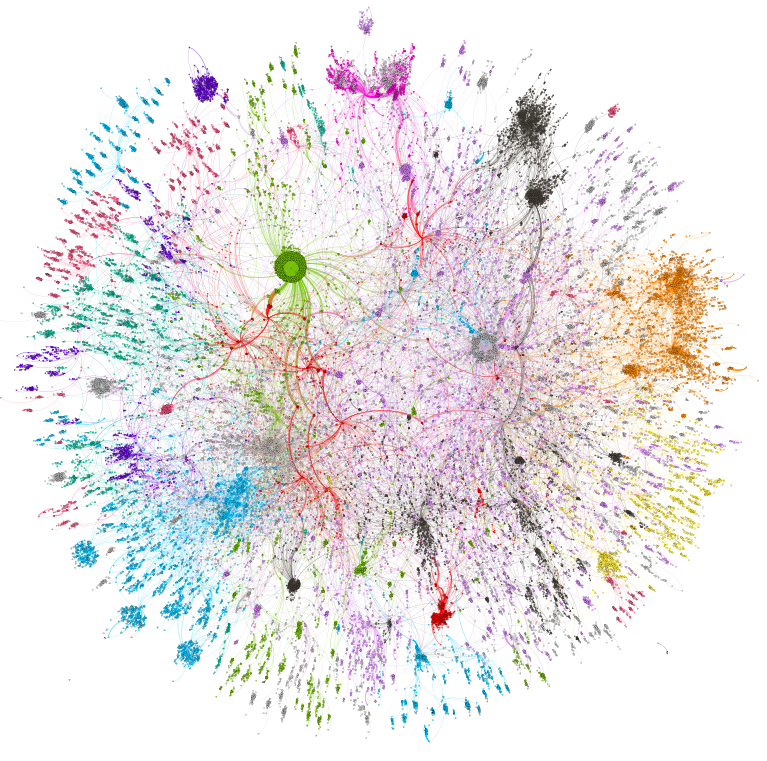
\includegraphics[width=1\columnwidth]{data.png}
    \caption{Graph of links between the pages, where the color represents the domain. Purple is gov.si, green is podatki.gov.si, light blue is gisportal.gov.si, black is evem.gov.si and orange is eugo.gov.si.}
    \label{fig1}
\end{figure}


\section{Conclusion}

The web crawler implementation was successful in obtaining the content of many of the gov.si websites.
It showed the robustness of it's implementation as the targeted websites had problems and inconsistencies.
It can be used as a general crawler although it is possible that it would require some more work to handle the possible exceptions that it hasn't encounter yet.

\bibliographystyle{IEEEtran}
\bibliography{main}

\end{document}
